% =====================================================================
% Relatório Técnico — Atividade 1 (AV1) — Projeto e Análise de Algoritmos
% PROCC/UFS 2026.2
%
% Compilação (não há LaTeX no ambiente onde este arquivo foi gerado;
% compile no Overleaf ou com uma distribuição TeX Live / MiKTeX):
%
%     pdflatex relatorio_av1.tex
%     pdflatex relatorio_av1.tex      % 2x, para numeração de páginas/refs
%
% Requer as figuras em figuras/crescimento_teorico.png e
% figuras/arvore_recorrencia.png (geradas por figuras/gerar_figuras.py).
% =====================================================================
\documentclass[11pt,a4paper]{article}

\usepackage[T1]{fontenc}
\usepackage[utf8]{inputenc}
\usepackage[brazilian]{babel}
\usepackage{lmodern}
\usepackage[a4paper,top=2.2cm,bottom=2.6cm,left=2.2cm,right=2.2cm]{geometry}
\usepackage{xcolor}
\usepackage{graphicx}
\usepackage{amsmath}
\usepackage{amssymb}
\usepackage{placeins}
\usepackage{booktabs}
\usepackage{array}
\usepackage{tabularx}
\usepackage{enumitem}
\usepackage{listings}
\usepackage{float}
\usepackage{mdframed}
\usepackage{titlesec}
\usepackage{fancyhdr}
\usepackage{lastpage}
\usepackage[hidelinks]{hyperref}

% ---------- cores ----------
\definecolor{azul}{HTML}{1F4E79}
\definecolor{azul2}{HTML}{2E5C8A}
\definecolor{laranja}{HTML}{C55A11}
\definecolor{verde}{HTML}{2E7D32}
\definecolor{fundo}{HTML}{F1F4F8}
\definecolor{fundolaranja}{HTML}{FFF6EF}
\definecolor{fundoverde}{HTML}{F0F7F0}
\definecolor{fundoazul}{HTML}{F3F7FC}
\definecolor{linha}{HTML}{C7CED6}
\definecolor{cinza}{HTML}{555555}

% ---------- espaçamento de parágrafo ----------
\setlength{\parindent}{0pt}
\setlength{\parskip}{6pt}
\linespread{1.05}

% ---------- títulos coloridos ----------
\titleformat{\section}{\normalfont\Large\bfseries\color{azul}}{\thesection.}{0.5em}{}
\titleformat{\subsection}{\normalfont\large\bfseries\color{azul2}}{\thesubsection}{0.5em}{}
\titlespacing*{\section}{0pt}{16pt}{6pt}

% ---------- rodapé ----------
\pagestyle{fancy}
\fancyhf{}
\renewcommand{\headrulewidth}{0pt}
\renewcommand{\footrulewidth}{0.4pt}
\fancyfoot[L]{\footnotesize\textcolor{cinza}{Projeto e Análise de Algoritmos --- AV1 $\cdot$ PROCC/UFS 2026.2}}
\fancyfoot[R]{\footnotesize\textcolor{cinza}{Página \thepage\ de \pageref{LastPage}}}

% ---------- caixas ----------
\newmdenv[linecolor=laranja,linewidth=3pt,topline=false,rightline=false,bottomline=false,
  backgroundcolor=fundolaranja,innerleftmargin=10pt,innerrightmargin=10pt,
  innertopmargin=8pt,innerbottommargin=8pt,skipabove=8pt,skipbelow=8pt]{nota}
\newmdenv[linecolor=verde,linewidth=3pt,topline=false,rightline=false,bottomline=false,
  backgroundcolor=fundoverde,innerleftmargin=10pt,innerrightmargin=10pt,
  innertopmargin=8pt,innerbottommargin=8pt,skipabove=8pt,skipbelow=8pt]{teo}
\newmdenv[linecolor=azul,linewidth=1pt,backgroundcolor=fundoazul,
  innerleftmargin=10pt,innerrightmargin=10pt,
  innertopmargin=8pt,innerbottommargin=8pt,skipabove=8pt,skipbelow=8pt]{inv}
\newmdenv[linecolor=laranja,linewidth=1pt,backgroundcolor=fundolaranja,
  innerleftmargin=10pt,innerrightmargin=10pt,
  innertopmargin=8pt,innerbottommargin=8pt,skipabove=8pt,skipbelow=8pt]{status}

% ---------- pseudocódigo (conteúdo em ASCII para compilar sem tropeços) ----------
\lstdefinestyle{pseudo}{
  basicstyle=\ttfamily\footnotesize,
  backgroundcolor=\color{fundo},
  frame=single, framesep=6pt, rulecolor=\color{linha},
  keywordstyle=\color{azul}\bfseries,
  commentstyle=\color{cinza}\itshape,
  morekeywords={funcao,para,ate,faca,se,entao,senao,enquanto,retorne},
  columns=fullflexible, breaklines=true, showstringspaces=false,
  xleftmargin=4pt, xrightmargin=4pt, aboveskip=8pt, belowskip=8pt,
}
\lstset{style=pseudo}

\newcolumntype{Y}{>{\raggedright\arraybackslash}X}

\hypersetup{pdftitle={Relatório Técnico AV1 - PAA 2026.2},
  pdfauthor={Equipe PAA UFS 2026.2}}

% =====================================================================
\begin{document}

% ---------------------------- CAPA ----------------------------
\begin{titlepage}
\thispagestyle{empty}
\centering
\vspace*{0.6cm}
{\normalsize\color{cinza}
Universidade Federal de Sergipe --- \textbf{\color{azul}PROCC}\\[2pt]
Projeto e Análise de Algoritmos $\cdot$ Período 2026.2\\[2pt]
Módulo I --- Fundamentos e Eficiência na Era dos Dados\par}

\vfill
{\color{laranja}\rule{0.7\textwidth}{2pt}}\par
\vspace{10pt}
{\large\color{laranja}\textbf{Atividade 1 (AV1) --- Relatório Técnico}}\par
\vspace{14pt}
{\Huge\bfseries\color{azul} Recuperação de contexto para IA generativa em materiais educacionais abertos\par}
\vspace{10pt}
{\large\color{cinza} Corretude, eficiência e recuperação de contexto:\\
um estudo comparativo de estratégias de ordenação e busca sobre um livro-texto aberto\par}
\vspace{8pt}
{\color{azul}\rule{0.7\textwidth}{2pt}}\par

\vspace{20pt}
{\large
João Cosme Sena Sá $\cdot$ Eduardo Henrique do Lago Silva $\cdot$ Helena Carvalho Leal\\[4pt]
Hernandison da Silva Bispo $\cdot$ Nadianne Maria dos Santos Galvão $\cdot$ Rafael Takeguma Goto\par}

\vspace{18pt}
\begin{tabular}{@{}r@{\quad}l@{}}
\textbf{Tema}            & 8 --- Materiais educacionais abertos\\
\textbf{Corpus}          & \emph{Pense Python} (tradução livre da 3\textsuperscript{a} ed. de \emph{Think Python})\\
\textbf{Repositório}     & \small\url{https://github.com/joaocss/PAA_UFS_2026_2_SenaSa_Joao_Bispo_Hernandison_Galvao_Nadianne_Goto_Rafael_Leal_Helena_Silva_Eduardo}\\
\textbf{Licença do código} & MIT $\cdot$ Versão/tag: v0.1.0\\
\textbf{Vídeo da atividade} & \emph{URL a preencher até 22/09/2026} (também em README, VIDEO.md e Classroom)\\
\end{tabular}

\vfill
{\footnotesize\color{cinza}
Documento gerado em 04/09/2026 $\cdot$ São Cristóvão, SE\\
Entrega dos artefatos até 23/09/2026 $\cdot$ Apresentação em 24/09/2026\par}
\end{titlepage}

% ---------------------------- STATUS ----------------------------
\begin{status}
\textbf{Estado desta versão do relatório.}
Este documento consolida a especificação formal, os algoritmos e pseudocódigos,
a prova de corretude, a análise no modelo RAM, as recorrências, a metodologia experimental, os resultados obtidos e a relação com RAG.

As figuras teóricas são explicitamente identificadas como diagramas ou curvas derivadas
das funções de complexidade, enquanto as tabelas e gráficos da Seção~\ref{sec:resultados} apresentam resultados experimentais obtidos a partir da execução do pipeline.

O experimento principal foi concluído com 3600 execuções mensuráveis, cobrindo quatro configurações, três tamanhos de corpus, 30 consultas, dois valores de $k$ e cinco repetições, além de duas execuções de aquecimento descartadas por cenário.
\end{status}

\tableofcontents

% ============================ 1 ============================
\section{Identificação da equipe}
Equipe de seis discentes do curso de Ciência da Computação (PROCC/UFS), na disciplina Projeto e
Análise de Algoritmos, período 2026.2. A modalidade é trabalho em equipe (5 a 7 integrantes).

\begin{table}[h]
\small\centering
\begin{tabularx}{\textwidth}{@{}p{6cm}Y@{}}
\toprule
\textbf{Integrante} & \textbf{Frente principal}\\
\midrule
João Cosme Sena Sá & Coordenação e entrega; dados de teste e pacote; índice invertido e busca binária no vocabulário (Config.~2)\\
Eduardo Henrique do Lago Silva & Experimentos, tabelas, gráficos e baseline de referência scikit-learn (Config.~4)\\
Helena Carvalho Leal & Consultas, julgamentos de relevância (qrels), métricas (Precision@k), relação com IA e limitações\\
Hernandison da Silva Bispo & Ingestão, normalização, fragmentação e manutenção do relatório\\
Nadianne Maria dos Santos Galvão & Corretude, modelo RAM, complexidade e recorrências\\
Rafael Takeguma Goto & Busca linear, Insertion Sort, Merge Sort, pontuação e consulta (Config.~1 e 3)\\
\bottomrule
\end{tabularx}
\end{table}

\begin{nota}
A divisão acima é a \textbf{divisão de frentes} acordada (\texttt{docs/CONTRIBUICOES.md}); a revisão de código, da prova e dos resultados é
responsabilidade coletiva. A tabela de contribuição individual \textbf{com evidências} é mantida em
\texttt{docs/CONTRIBUICOES.md} e resumida na Seção~\ref{sec:contrib}.
\end{nota}

% ============================ 2 ============================
\section{Tema, corpus e fonte}
O tema é o de número 8 do enunciado, \textbf{materiais educacionais abertos}. O corpus é o livro
\emph{Pense Python}, tradução livre da 3\textsuperscript{a} edição de \emph{Think Python}, de Allen
B. Downey, traduzida por Rodrigo Castelan Carlson --- conteúdo didático público de introdução à
programação em Python, sem qualquer dado sensível, pessoal ou sigiloso.

\begin{table}[h]
\small\centering
\begin{tabularx}{\textwidth}{@{}p{4.2cm}Y@{}}
\toprule
\textbf{Campo} & \textbf{Registro}\\
\midrule
Nome & \emph{Pense Python} --- tradução livre da 3\textsuperscript{a} ed. de \emph{Think Python}\\
Autor / Tradução & Allen B. Downey / Rodrigo Castelan Carlson\\
Fonte & \url{https://rodrigocarlson.github.io/PensePython3ed/} ; \url{https://github.com/rodrigocarlson/PensePython3ed}\\
Commit de referência & \texttt{cfde2c450bf4f2ea65326da88e9968f400597e92} (branch \texttt{main})\\
Recorte & 21 notebooks Jupyter: prefácio, introdução e capítulos 1 a 19 (\texttt{capitulos/*.ipynb})\\
Tamanho auditado & 817.578 bytes $\cdot$ 2.789 células $\cdot$ $\approx$73.867 palavras\\
SHA-256 do recorte & \texttt{2010626258\dots5768dc5} (agregado; ver \texttt{data/corpus\_manifest.csv})\\
Idioma & Português brasileiro (com estrangeirismos técnicos do Python/Jupyter)\\
Licença do texto / código & CC BY-NC-SA 4.0 / MIT\\
Data de acesso & 02/09/2026 (aquisição registrada); planejamento em 01/09/2026\\
Dados sensíveis & Nenhum --- conteúdo didático público\\
\bottomrule
\end{tabularx}
\end{table}

\begin{nota}
\textbf{Corpus não versionado, mas reprodutível.} Como a licença do texto é não comercial e com
compartilhamento pelas mesmas condições (CC BY-NC-SA), o texto não é redistribuído no repositório
(cujo código é MIT). O script \texttt{scripts/baixar\_corpus.py} baixa o material no commit fixado e
\texttt{data/corpus\_manifest.csv} guarda o SHA-256 de cada notebook e um \textbf{hash agregado do
recorte}, permitindo conferir que qualquer download reproduz o mesmo conjunto auditado. Trechos
citados preservam atribuição ao autor e ao tradutor.
\end{nota}

\textbf{Pergunta(s) de recuperação.} As consultas seguem o formato ``tira-dúvidas'' de um estudante
sobre o livro, por exemplo: \emph{``como funciona um laço \texttt{for} em Python?''},
\emph{``o que é uma função recursiva?''}, \emph{``como tratar exceções com \texttt{try} e
\texttt{except}?''}. O conjunto completo de 30 consultas está em \texttt{data/queries.csv}, redigido
\textbf{antes} de qualquer resultado ser observado.

% ============================ 3 ============================
\section{Repositório, licença, versão e data de acesso}
\begin{table}[h]
\small\centering
\begin{tabularx}{\textwidth}{@{}p{4.2cm}Y@{}}
\toprule
\textbf{Item} & \textbf{Registro}\\
\midrule
URL do repositório & \url{https://github.com/joaocss/PAA_UFS_2026_2_SenaSa_Joao_Bispo_Hernandison_Galvao_Nadianne_Goto_Rafael_Leal_Helena_Silva_Eduardo}\\
Licença do código & MIT (arquivo \texttt{LICENSE})\\
Versão / tag & v0.1.0 (\texttt{CITATION.cff}, \texttt{date-released: 2026-09-03})\\
Commit/tag/release do relatório & \emph{a fixar na entrega final (tag da release de 23/09/2026)}\\
Data de acesso ao corpus & 02/09/2026 (a reconfirmar no dia da aquisição)\\
Ambiente travado & \texttt{requirements.lock}: pytest 8.3.4, scikit-learn 1.6.1, matplotlib 3.10.0, numpy 2.2.2\\
\bottomrule
\end{tabularx}
\end{table}
O repositório não contém chaves, senhas, tokens, dados pessoais ou artefatos sem licença compatível.
Arquivos grandes são controlados por \texttt{.gitignore}; as instruções de obtenção e reprodução
estão no \texttt{README.md}.

% ============================ 4 ============================
\section{Definição formal do problema}\label{sec:def}
O protótipo é um \textbf{recuperador de contexto}: dada uma consulta, devolve os trechos mais
relevantes do corpus, ordenados por relevância. Não é um chatbot; o interesse está nas operações
algorítmicas anteriores à geração de texto.

\subsection{Entradas e saída}
\begin{itemize}[leftmargin=1.4em,itemsep=2pt]
\item \textbf{Corpus} $C = \langle c_1,\dots,c_N\rangle$: sequência de $N$ chunks. Cada chunk $c_i$ tem
um \texttt{chunk\_id} textual único, um \texttt{source\_order} $id_i$ inteiro único em $0..N-1$ (usado
no desempate), o texto normalizado e $\text{origem}_i=(\text{notebook},\text{seção},\text{offset})$.
\item \textbf{Consulta} $q$: cadeia em português; após normalização vira um multiconjunto de $m$ termos.
\item $\mathbf{k}\in\mathbb{N}$: número máximo de trechos a devolver.
\item \textbf{Saída} $R$: sequência de até $k$ chunks de $C$, sem repetição, ordenada de forma não
crescente pela função de relevância.
\end{itemize}
\subsection{Função de relevância}
A pontuação é \textbf{TF-IDF} lexical, definida pela equipe e usada de forma idêntica nas três
configurações obrigatórias:
\begin{align*}
\mathrm{tf}(t,c) &= 1 + \ln f_{t,c}
\quad (\text{se } f_{t,c}>0;\ \text{senão } 0),\\
\mathrm{idf}(t) &= \ln\!\left(\frac{N+1}{\mathrm{df}(t)+1}\right)+1,\\[2pt]
\mathrm{score}(q,c) &=
\sum_{t\in \mathrm{Termos}(q)}
qtf_t \cdot \mathrm{tf}(t,c)\cdot\mathrm{idf}(t).
\end{align*}

$qtf_t$ representa a frequência do termo $t$ na consulta,
$f_{t,c}$ é a frequência do termo $t$ no chunk $c$ e
$\mathrm{df}(t)$ é o número de chunks que contêm $t$.
Termos ausentes do vocabulário não contribuem para a pontuação.

A suavização adotada para o IDF segue a mesma forma utilizada pela configuração de referência com scikit-learn, enquanto a ponderação TF-IDF da implementação própria foi mantida explícita para permitir a comparação entre as configurações.

A \textbf{ordem total}
$\preceq$ é:
\[
c_a \preceq c_b \iff \mathrm{score}(q,c_a) > \mathrm{score}(q,c_b)\ \lor\
\big(\text{scores iguais}\ \wedge\ id_a < id_b\big),
\]
onde $id$ denota o \texttt{source\_order} do chunk. O desempate determinístico por \texttt{source\_order}
crescente garante que o resultado independe da ordem de entrada e da configuração usada.

\subsection{Pré-condições, pós-condições e casos de borda}
\begin{table}[h]
\small\centering
\begin{tabularx}{\textwidth}{@{}p{2.8cm}Y@{}}
\toprule
\textbf{Categoria} & \textbf{Especificação}\\
\midrule
Pré-condições & $N\ge0$; $k\ge0$; todo score é real finito; os \texttt{source\_order} são únicos; $\preceq$ é ordem total.\\
Pós-condições & Seja $n'$ o número de chunks com score $>0$. Então $|R|=\min(k,n')$; todo elemento de
$R$ pertence a $C$ e é único; $R$ está ordenado por $\preceq$; e não existe chunk fora de $R$ com
relevância maior (por $\preceq$) que qualquer elemento de $R$ --- ou seja, $R$ são os $\min(k,n')$ melhores.\\
Casos de borda & consulta vazia $\to R=\langle\rangle$; $k=0\to R=\langle\rangle$; $k>n'\to$ devolve
os $n'$ com score $>0$; todos os scores 0 $\to R=\langle\rangle$; empates $\to$ resolvidos por \texttt{source\_order};
termo fora do vocabulário $\to$ ignorado.\\
Hipótese sobre os dados & Para a vantagem do índice invertido (Config.~2) supõe-se \textbf{esparsidade}:
$\mathrm{df}\ll N$ para os termos típicos. A corretude não depende dessa hipótese; apenas a eficiência.\\
\bottomrule
\end{tabularx}
\end{table}

% ============================ 5 ============================
\section{Representação dos dados e estratégia de chunking}
\subsection{Normalização}
Deliberadamente simples, para poder ser auditada:
\begin{itemize}[leftmargin=1.4em,itemsep=2pt]
\item \textbf{Células de texto (Markdown):} NFKC, minúsculas, separação controlada da pontuação e
compactação de espaços; \textbf{acentos preservados}.
\item \textbf{Células de código:} fonte intacta, com uma visão lexical à parte (tokens), sem alterar indentação.
\item \textbf{Stopwords não são removidas} na configuração principal: em português isso apagaria termos
funcionais que mudam o sentido de consultas como \emph{``diferença entre \texttt{while} e \texttt{for}''}.
\item Saídas de execução das células são descartadas.
\end{itemize}

\subsection{Segmentação (chunking)}
Respeita a hierarquia do livro --- notebook, título e seção --- e \textbf{nunca mistura} célula de
texto com célula de código no mesmo chunk. A configuração principal usa \textbf{256 tokens} com
\textbf{sobreposição de 32}, produzindo cerca de \textbf{2737 chunks}. As configurações 128/16 e
512/64 entram apenas no experimento de sensibilidade.

\subsection{Representações computacionais}
\begin{itemize}[leftmargin=1.4em,itemsep=2pt]
\item \textbf{Saco de palavras / TF-IDF:} cada chunk é um vetor esparso de pesos TF-IDF sobre $V$.
\item \textbf{Índice invertido (Config.~2):} mapa termo $\to$ lista de \emph{postings} $(id, f_{t,c})$,
com o \textbf{vocabulário em vetor ordenado} para permitir \textbf{busca binária} por termo.
\end{itemize}
\begin{nota}
\textbf{Riscos conhecidos.} A tradução carrega termos em inglês do Python/Jupyter (ex.: \emph{loop},
\emph{string}), o que afeta consultas com e sem estrangeirismos; um único livro introdutório não
representa todo o universo dos materiais educacionais abertos --- os resultados valem como
\textbf{estudo de caso}.
\end{nota}

% ============================ 6 ============================
\section{Algoritmos e pseudocódigo}
Os algoritmos obrigatórios são cobertos assim: \textbf{busca linear} na pontuação de todos os chunks;
\textbf{ordenação} por Insertion Sort e Merge Sort da equipe; \textbf{busca binária} no vocabulário
do índice invertido; \textbf{divisão e conquista} pelo próprio Merge Sort; e \textbf{comparação com
biblioteca} pelo TF-IDF do scikit-learn, usado apenas como referência (Config.~4).

\subsection{Busca linear com pontuação (comum a C1 e C3)}
\begin{lstlisting}
funcao PontuarLinear(q, C, idf):
  candidatos <- lista vazia
  para cada chunk c em C faca            # N iteracoes
    s <- 0
    para cada termo t em q faca          # m iteracoes
      se t in c.termos entao             # teste O(1) via hash
        s <- s + tf(t, c) * idf[t]
    se s > 0 entao candidatos.anexar( (s, c.id, c) )
  retorne candidatos
\end{lstlisting}

\subsection{Insertion Sort --- Config.~1}
\begin{lstlisting}
funcao InsertionSort(A, precede):
  para i <- 1 ate |A|-1 faca
    chave <- A[i];  j <- i - 1
    enquanto j >= 0 e A[j] sucede chave faca   # desloca os maiores
      A[j+1] <- A[j];  j <- j - 1
    A[j+1] <- chave
  retorne A
\end{lstlisting}

\subsection{Merge Sort --- Config.~3 e estratégia de divisão e conquista}
\begin{lstlisting}
funcao MergeSort(A, precede):
  se |A| <= 1 entao retorne A            # caso base
  meio <- floor(|A| / 2)
  E <- MergeSort(A[0 .. meio-1])         # T(N/2)
  D <- MergeSort(A[meio .. |A|-1])       # T(N/2)
  retorne Merge(E, D)                    # Theta(N)

funcao Merge(E, D):
  O <- lista vazia;  i <- 0;  j <- 0
  enquanto i < |E| e j < |D| faca
    se E[i] precede-ou-igual D[j] entao         # estavel: empate -> E
      O.anexar(E[i]); i <- i + 1
    senao
      O.anexar(D[j]); j <- j + 1
  O.anexar(restante de E a partir de i)
  O.anexar(restante de D a partir de j)
  retorne O
\end{lstlisting}

\subsection{Índice invertido e busca binária --- Config.~2}
\begin{lstlisting}
funcao BuscaBinaria(vocab, t):           # vocab = vetor ORDENADO de termos
  lo <- 0; hi <- |vocab| - 1
  enquanto lo <= hi faca
    mid <- floor((lo + hi) / 2)
    se vocab[mid] = t entao retorne mid
    senao se vocab[mid] < t entao lo <- mid + 1
    senao hi <- mid - 1
  retorne NAO_ENCONTRADO

funcao BuscarIndexado(q, indice, estatisticas):
  termos <- termos distintos normalizados de q
  posicoes <- lista vazia

  para cada termo t em termos faca
    p <- BuscaBinaria(indice.vocabulario, t)   # Theta(log V)
    se p != NAO_ENCONTRADO entao
      posicoes <- UnirPostings(
        posicoes,
        indice.postings[p]
      )

  candidatos <- lista vazia

  para cada posicao em posicoes faca
    c <- indice.chunks[posicao]
    s <- RelevanceScore(q, c, estatisticas)

    se s > 0 entao
      candidatos.anexar((c, s))

  retorne MergeSort(candidatos)          # ordena apenas os candidatos
\end{lstlisting}

\subsection{Seleção dos $k$ melhores (comum a todas)}
\begin{lstlisting}
funcao TopK(resultados_ordenados, k):
  se k <= 0 entao
    retorne lista vazia

  candidatos <- lista vazia

  para cada (chunk, score) em resultados_ordenados faca
    se score > 0 entao
      candidatos.anexar((chunk, score))

  retorne os primeiros min(k, |candidatos|) elementos
\end{lstlisting}
Como a lista já está ordenada pela relação $\preceq$, a filtragem preserva essa
ordem. Assim, os primeiros $\min(k,|candidatos|)$ elementos correspondem aos
 $k$ resultados válidos mais relevantes.

% ============================ 7 ============================
\section{Justificativa de corretude}\label{sec:corretude}
Provamos a corretude do \textbf{Merge Sort} (Config.~3 e núcleo da Config.~2), por indução forte no
tamanho da entrada, apoiada em um invariante de laço para o \texttt{Merge}. O texto completo está em
\texttt{docs/CORRETUDE.md}.

\begin{teo}
\textbf{\color{verde}Teorema.} Dada uma lista finita $A$ de chunks com identificadores únicos e a
ordem total $\preceq$ (score decrescente; empate por $id$ crescente), \texttt{MergeSort(A,$\preceq$)}
\textbf{termina} e devolve uma \textbf{permutação de $A$ ordenada} por $\preceq$.
\end{teo}

\textbf{Hipóteses.}
\begin{itemize}[leftmargin=1.4em,itemsep=1pt]
\item $A$ é finita; cada elemento tem score real finito e $id$ único.
\item $\preceq$ é ordem total: reflexiva, antissimétrica (pelo desempate por $id$ único) e transitiva.
\item A comparação de dois elementos custa $\Theta(1)$.
\end{itemize}

\textbf{Lema (corretude do \texttt{Merge}) --- invariante de laço.}
\begin{inv}
\textbf{Invariante.} No início de cada iteração do laço \textbf{enquanto} de \texttt{Merge(E,D)}, com
$E$ e $D$ já ordenados por $\preceq$: (i)~a saída $O$ está ordenada por $\preceq$; (ii)~$O$ contém
exatamente os elementos já consumidos de $E$ (índices $<i$) e de $D$ (índices $<j$); e (iii)~todo
elemento de $O$ é $\preceq$ a qualquer elemento ainda não consumido de $E$ ou $D$.
\end{inv}
\begin{itemize}[leftmargin=1.4em,itemsep=1pt]
\item \textbf{Inicialização.} $O=\langle\rangle$ e $i=j=0$; (i)--(iii) valem vacuamente.
\item \textbf{Manutenção.} O algoritmo escolhe o menor entre $E[i]$ e $D[j]$ (empate a favor de $E$).
Como $E$ e $D$ estão ordenados, o escolhido $x$ é $\preceq$ a todos os não consumidos; pode ser
anexado ao fim de $O$ preservando (i) e (iii). O contador avança, mantendo (ii).
\item \textbf{Término.} Cada iteração consome um elemento; o laço executa no máximo $|E|+|D|$ vezes.
Os elementos restantes da lista não esgotada já são, por (iii), $\preceq$ a nada em $O$ e estão em
ordem; anexá-los mantém $O$ ordenado. Ao final, $O$ é uma permutação ordenada de $E\cup D$.
\end{itemize}

\textbf{Indução no tamanho de $A$.}
\begin{itemize}[leftmargin=1.4em,itemsep=1pt]
\item \textbf{Base ($|A|\le1$).} Devolvida como está: trivialmente ordenada e permutação de si mesma.
\item \textbf{Hipótese de indução.} \texttt{MergeSort} é correto para toda entrada de tamanho $<n$.
\item \textbf{Passo ($|A|=n>1$).} $A$ é dividida em $E$ ($\lfloor n/2\rfloor$) e $D$
($n-\lfloor n/2\rfloor$), ambas de tamanho $<n$. Por hipótese de indução, as chamadas recursivas
devolvem permutações ordenadas de $E$ e de $D$. Pelo Lema, \texttt{Merge(E,D)} devolve uma permutação
ordenada de $E\cup D$, que é $A$ a menos de reordenação. $\blacksquare$
\end{itemize}

\textbf{Término da recursão.} Os tamanhos decrescem estritamente ($\lfloor n/2\rfloor<n$ e
$n-\lfloor n/2\rfloor<n$ para $n>1$) e atingem o caso base; logo a recursão é finita.

\textbf{Estabilidade e desempate.} O \texttt{Merge} anexa de $E$ em caso de empate, tornando a
ordenação \textbf{estável}. Como os $id$ são únicos e entram em $\preceq$, não há empates verdadeiros
entre chunks distintos: a saída é \textbf{determinística}, qualquer que seja a ordem de entrada ou a
configuração (C1, C2 ou C3).

\begin{teo}
\textbf{\color{verde}Corolário (top-$k$).} Se $A$ está ordenada por $\preceq$, seus primeiros
$\min(k,|A|)$ elementos são exatamente os $k$ maiores segundo $\preceq$. Logo \texttt{TopK} aplicado
à saída do \texttt{MergeSort} devolve os $k$ chunks mais relevantes, cumprindo a pós-condição da
Seção~\ref{sec:def}.
\end{teo}

\textbf{Limites do argumento e casos em que não se aplica.}
\begin{itemize}[leftmargin=1.4em,itemsep=1pt]
\item Garante \textbf{ordenação correta e término}, não que o TF-IDF corresponda à intenção de quem
consultou: relevância lexical é um \emph{proxy} imperfeito (Seções~\ref{sec:rag} e~\ref{sec:limit}).
\item Se algum score for indefinido (NaN) ou o comparador não for transitivo, $\preceq$ deixa de ser
ordem total e o teorema não se aplica.
\item Se os $id$ não forem únicos, o desempate falha e a saída pode deixar de ser determinística.
\item A prova não trata de precisão de ponto flutuante; scores muito próximos podem ser tratados como
empate e decididos pelo \texttt{source\_order} --- comportamento coberto pelos testes.
\end{itemize}

\subsection{Validação prática da ordenação}
Como complemento à prova, a relação de ordem $\preceq$ usada em todas as configurações é validada
diretamente em \texttt{tests/unit/test\_sort\_key.py}, sobre a função \texttt{sort\_key} de
\texttt{src/paa\_context/sort\_key.py}, que estabelece maior \texttt{score} primeiro e, em empate,
menor \texttt{source\_order}. Três testes cobrem os pilares do argumento:
\begin{itemize}[leftmargin=1.4em,itemsep=1pt]
\item \texttt{test\_maior\_score\_vem\_primeiro}: prioridade do maior \texttt{score};
\item \texttt{test\_empate\_usa\_menor\_source\_order}: critério de desempate por \texttt{source\_order};
\item \texttt{test\_ordem\_transitiva}: transitividade da relação (condição para $\preceq$ ser ordem total).
\end{itemize}
Os três passam isoladamente e a suíte completa do projeto é executada e aprovada
(118 testes aprovados na suíte completa do projeto, incluindo os três testes específicos de \texttt{sort\_key}). Esta subseção consolida a análise de corretude conduzida por Nadianne Galvão (\texttt{docs/CORRETUDE.md} e o documento de corretude, RAM, complexidade e
recorrências).

% ============================ 8 ============================
\section{Análise no modelo RAM}
\subsection{Parâmetros}
\begin{table}[h]
\small\centering
\begin{tabularx}{\textwidth}{@{}p{1.6cm}Y@{}}
\toprule
\textbf{Símbolo} & \textbf{Significado}\\
\midrule
$N$ & número de chunks (2737 na configuração principal)\\
$V$ & tamanho do vocabulário (termos distintos)\\
$L$ & total de tokens do corpus\\
$m$ & número de termos da consulta\\
$\ell$ & número de termos do chunk analisado\\
$k$ & número de resultados retornados\\
$C_q$ & número de chunks candidatos (score $>0$) para a consulta $q$\\
$P$ & tamanho total das listas de postings percorridas $=\sum_{t\in q}\mathrm{df}(t)$\\
$r$ & número de repetições experimentais\\
\bottomrule
\end{tabularx}
\end{table}

\subsection{Operações elementares e custo por algoritmo}
Contam-se como operações elementares: comparação de chaves, acesso a vetor/lista, atribuição,
incremento, chamada recursiva, consulta a tabela de dispersão e atualização de estrutura.

\textbf{Insertion Sort (sobre $C_q$ candidatos).} O laço externo executa $C_q-1$ vezes; o interno
desloca, no pior caso, todos os já ordenados. Comparações
$\sum_{i=1}^{C_q-1} i = C_q(C_q-1)/2$ no pior caso, com igual ordem de acessos e atribuições. Como a implementação cria uma cópia da lista de entrada antes da ordenação, o espaço adicional é $O(C_q)$.

\textbf{Merge Sort (sobre $C_q$ candidatos).} Cada nível percorre todos os elementos uma vez
($\Theta(C_q)$ por nível) e há $\lceil\log_2 C_q\rceil$ níveis, dando $\Theta(C_q\log C_q)$
comparações. Espaço $\Theta(C_q)$ pelas listas auxiliares.

\textbf{Custo do pipeline por configuração.}
\begin{table}[h]
\small\centering
\begin{tabularx}{\textwidth}{@{}p{3.4cm}YYY@{}}
\toprule
\textbf{Etapa} & \textbf{C1 (lin.+Insertion)} & \textbf{C2 (índice+bin.+Merge)} & \textbf{C3 (lin.+Merge)}\\
\midrule
Pontuação / candidatos
& $\Theta(N(m+\ell))$
& $O(m\log V + mP + C_q(m+\ell))$
& $\Theta(N(m+\ell))$\\
Seleção top-$k$ & $\Theta(C_q)$ & $\Theta(C_q)$ & $\Theta(C_q)$\\
Espaço adicional (consulta) & $\Theta(C_q)$ & $\Theta(V+P_{\text{tot}})+\Theta(C_q)$ & $\Theta(C_q)$\\
\bottomrule
\end{tabularx}
\end{table}
\begin{nota}
\textbf{Fatores fora do modelo RAM.} O modelo ignora hierarquia de cache, custo de E/S ao ler os
notebooks, alocação de memória, coletor de lixo do Python e a diferença entre código interpretado
(C1--C3) e rotinas vetorizadas em C/NumPy (Config.~4). Por isso a Seção~\ref{sec:resultados} mede
tempo de parede além de contar operações. 
\end{nota}

% ============================ 9 ============================
\section{Melhor, pior e caso médio}
\begin{table}[h]
\small\centering
\begin{tabularx}{\textwidth}{@{}p{3.4cm}YYYp{1.5cm}@{}}
\toprule
\textbf{Algoritmo} & \textbf{Melhor} & \textbf{Pior} & \textbf{Médio} & \textbf{Espaço}\\
\midrule
Busca/pontuação linear & $\Theta(N(m+\ell))$ & $\Theta(N(m+\ell))$ & $\Theta(N(m+\ell))$ & $\Theta(C_q)$\\
Insertion Sort & $\Theta(n)$ & $\Theta(n^2)$ & $\Theta(n^2)$ & $O(n)$\\
Merge Sort & $\Theta(n\log n)$ & $\Theta(n\log n)$ & $\Theta(n\log n)$ & $\Theta(n)$\\
Busca binária (por termo) & $\Theta(1)$ & $\Theta(\log V)$ & $\Theta(\log V)$ & $\Theta(1)$\\
Consulta via índice (C2)
& $O(m\log V + mP + C_q(m+\ell) + C_q\log C_q)$
& $O(m\log V + mP + C_q(m+\ell) + C_q\log C_q)$
& $O(m\log V + mP + C_q(m+\ell) + C_q\log C_q)$
& $\Theta(V+P_{\text{tot}}+C_q)$\\
\bottomrule
\end{tabularx}
\end{table}

Onde $n=C_q$ é o número de candidatos a ordenar e $\ell$ é o número de termos do chunk analisado.

\begin{itemize}[leftmargin=1.4em,itemsep=2pt]
\item \textbf{Insertion Sort} só é competitivo com $C_q$ pequeno ou lista quase ordenada; melhor caso linear quando não há deslocamento.

\item \textbf{Merge Sort} tem custo $\Theta(n\log n)$ \textbf{garantido} nos três casos ---
escolha segura para a comparação.

\item \textbf{Na Configuração 2}, o custo depende fortemente da frequência dos termos consultados.
Quando as listas de postings são pequenas, tanto $P$ quanto $C_q$ permanecem reduzidos, diminuindo o trabalho de união, pontuação e ordenação dos candidatos. No pior caso, termos muito frequentes podem fazer $C_q$ se aproximar de $N$, reduzindo a vantagem do índice em relação à busca linear.
\end{itemize}

% ============================ 10 ============================
\section{Recorrências}
\subsection{Merge Sort}
\[ T(N) = 2\,T(N/2) + \Theta(N),\qquad T(1)=\Theta(1). \]
\textbf{Origem dos termos:} o fator \textbf{2} vem das duas chamadas recursivas (metades $E$ e $D$);
cada $T(N/2)$ ordena uma metade; o termo $\Theta(N)$ é o \texttt{Merge}, que percorre linearmente as
duas metades. Pela \textbf{árvore de recorrência} (Figura~\ref{fig:arvore}), cada um dos
$\lceil\log_2 N\rceil+1$ níveis realiza trabalho $\Theta(N)$, somando $\Theta(N\log N)$. Pelo
\textbf{Teorema Mestre}, com $a=2$, $b=2$, tem-se $N^{\log_b a}=N^1$ e $f(N)=\Theta(N)$: caso~2,
dando $T(N)=\Theta(N\log N)$.

\begin{figure}[H]\centering
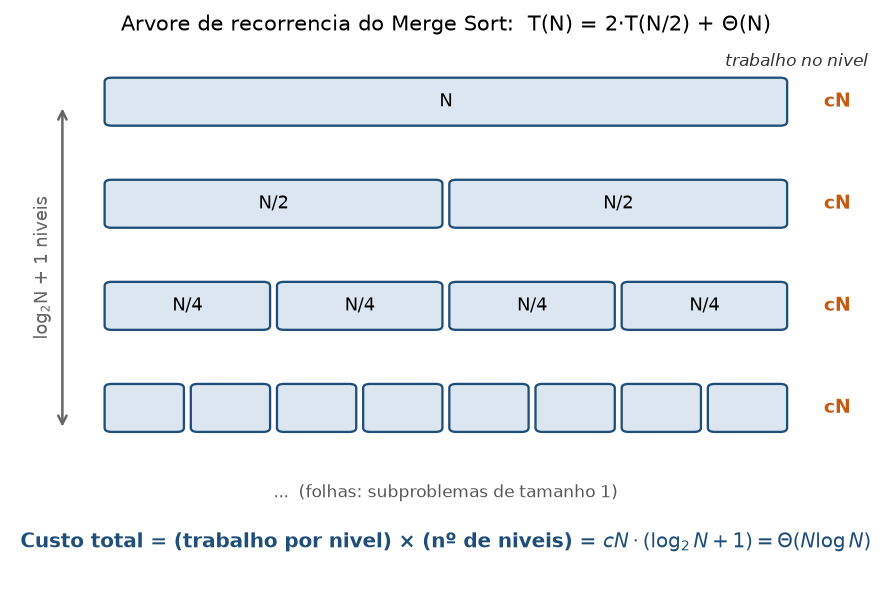
\includegraphics[width=0.86\textwidth]{figuras/arvore_recorrencia.png}
\caption{Árvore de recorrência de $T(N)=2\,T(N/2)+\Theta(N)$: trabalho $\Theta(N)$ por nível e
$\log_2 N + 1$ níveis, resultando em $\Theta(N\log N)$. Diagrama teórico.}
\label{fig:arvore}
\end{figure}

\subsection{Busca binária}
\[ T(V) = T(V/2) + \Theta(1),\qquad T(1)=\Theta(1). \]
\textbf{Origem dos termos:} embora a implementação da busca binária seja iterativa,
a recorrência $T(V)=T(V/2)+\Theta(1)$ modela a redução do intervalo de busca
a cada iteração. Em cada passo, aproximadamente metade do vocabulário é descartada, enquanto o trabalho para calcular o ponto médio, comparar com \texttt{vocab[mid]} e atualizar os limites é constante, representado por $\Theta(1)$. Assim, após aproximadamente $\log_2 V$ reduções, o intervalo atinge tamanho unitário, resultando em $T(V)=\Theta(\log V)$. 
A mesma recorrência também pode ser resolvida pelo Teorema Mestre, com $a=1$ e $b=2$, obtendo-se igualmente $T(V)=\Theta(\log V)$.

% ============================ 11 ============================
\section{Metodologia experimental}
\subsection{Configurações comparadas}
\begin{table}[h]
\small\centering
\begin{tabularx}{\textwidth}{@{}p{2.4cm}Yp{4.2cm}@{}}
\toprule
\textbf{Config.} & \textbf{Descrição} & \textbf{Papel}\\
\midrule
\textbf{C1} baseline & Varredura linear + Insertion Sort (equipe) & Baseline sem estrutura\\
\textbf{C2} indexada & Índice invertido + busca binária + Merge Sort dos candidatos & Busca indexada/otimizada\\
\textbf{C3} ordenada & Varredura linear + Merge Sort (equipe) & Divisão e conquista na ordenação\\
\textbf{C4} referência & TF-IDF do scikit-learn & Somente baseline externo\\
\bottomrule
\end{tabularx}
\end{table}
As três obrigatórias usam \textbf{os mesmos dados e a mesma função de pontuação}; diferem só na
estrutura de busca e na ordenação. Consequência para a validação: \textbf{C1, C2 e C3 devem produzir
listas ranqueadas idênticas} (mesma ordem $\preceq$), diferindo apenas em custo --- um teste de
consistência forte. A Config.~4 pode divergir por usar normalização L2 e TF sublinear próprias.

\subsection{Cargas, repetições e execuções}

O experimento principal compreende
\textbf{4 configurações $\times$ 3 tamanhos de corpus $\times$ 30 consultas
$\times$ 2 valores de $k$ $\times$ 5 repetições $=$ 3600 execuções mensuráveis}.
Antes das repetições medidas, são realizadas duas execuções de aquecimento por cenário, que são descartadas.

Os três tamanhos de corpus correspondem a aproximadamente 25\% (684 chunks),
50\% (1368 chunks) e 100\% (2737 chunks), obtidos por subamostragem determinística por capítulo com semente fixa. Cada consulta é executada para $k=5$ e $k=10$.

Ao final das 3600 execuções, não foram observadas divergências entre os rankings
produzidos por C1, C2 e C3. Esse resultado reforça que as três configurações
implementadas preservam a mesma saída de recuperação sob a mesma função de relevância e o mesmo critério de ordenação, diferindo principalmente no custo computacional.

\subsection{Métricas registradas}
\begin{itemize}[leftmargin=1.4em,itemsep=1pt]
\item Tempo de ingestão; de ordenação/construção de índice; de consulta; total.
\item Memória aproximada (via \texttt{tracemalloc} e RSS).
\item \textbf{Número de comparações}, por contador instrumentado.
\item Tamanho do corpus, número de chunks e $k$.
\item Precision@$k$ contra a referência manual de relevância construída para as 30 consultas.
\item Taxa de falhas, resultados vazios ou irrelevantes; custo e limitações.
\end{itemize}

\subsection{Reprodutibilidade}
Todo o pipeline roda com \texttt{python scripts/reproduzir\_tudo.py} (download $\to$ normalização
$\to$ chunking $\to$ experimentos $\to$ figuras). Os scripts são \textbf{idempotentes}. Cada execução
registra em \texttt{experimentos/logs}: hostname, processador, memória, SO, versão do Python, versões
das bibliotecas, commit e a linha de comando completa. As consultas e a referência manual de relevância foram definidas antes da análise dos resultados,
reduzindo o risco de viés de seleção.

\subsection{Referência de relevância}

A avaliação da qualidade utiliza uma referência de relevância construída manualmente para as 30 consultas. Para cada consulta foi definido um conjunto de chunks considerados pertinentes, acompanhado de justificativa. No cálculo de Precision@$k$, os chunks presentes nessa referência são tratados como relevantes e os demais como não relevantes.
% ============================ 12 ============================
\section{Resultados e gráficos}\label{sec:resultados}
\begin{figure}[H]\centering
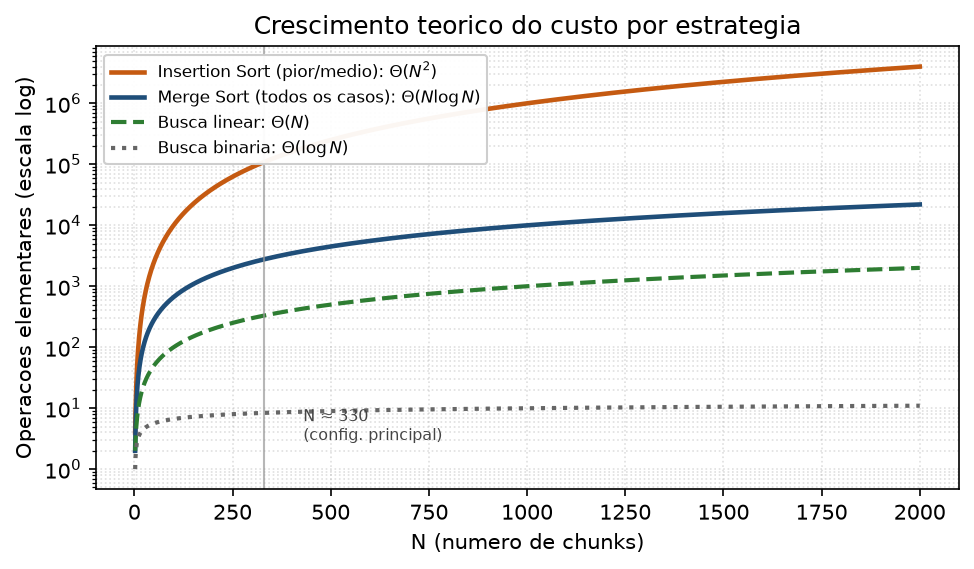
\includegraphics[width=0.9\textwidth]{figuras/crescimento_teorico.png}
\caption{Crescimento teórico do número de operações elementares em função de $N$ (escala log em $y$).
A separação entre $\Theta(N^2)$ (Insertion), $\Theta(N\log N)$ (Merge) e $\Theta(\log N)$ (busca
binária) motiva as três configurações. Curvas teóricas, não medições.}
\label{fig:crescimento}
\end{figure}


\subsection{Tempo por etapa e configuração}

\begin{table}[h]
\small\centering
\begin{tabularx}{\textwidth}{@{}llYYYYY@{}}
\toprule
\textbf{Config.} & \textbf{N} & \textbf{Ingestão (ms)} &
\textbf{Ord./índice (ms)} & \textbf{Consulta (ms)} &
\textbf{Total (ms)} & \textbf{Comparações}\\
\midrule
C1 & 2737 & 39,31 & 63,87 & 128,03 & 166,81 & 461702\\
C2 & 2737 & 39,35 & 40,96 & 47,14 & 127,98 & 13039\\
C3 & 2737 & 39,47 & 2,34 & 65,55 & 105,95 & 12746,5\\
C4 (ref.) & 2737 & 39,38 & 47,22 & 0,39 & 87,25 & n/a\\
\bottomrule
\end{tabularx}
\caption{Tempos medianos por etapa e contagem de comparações para o corpus completo.}
\label{tab:tempos-config}
\end{table}

Os resultados mostram que C1 apresentou o maior tempo total entre as três
implementações próprias, associado principalmente ao custo da ordenação por
Insertion Sort. C2 reduziu o tempo de consulta em relação a C1, embora tenha
incorporado o custo de construção do índice. C3 apresentou o menor tempo total
entre C1--C3 no corpus completo. A configuração C4 apresentou o menor tempo
total mediano, sendo utilizada apenas como referência externa baseada em biblioteca.
\begin{figure}[H]
\centering

\includegraphics[width=0.9\textwidth]{figuras/decomposicao_do_tempo.png}
\caption{Decomposição do tempo mediano por etapa para o corpus completo
($N=2737$). Em C1, a ordenação representa parcela relevante do custo;
C2 incorpora o custo de construção do índice; C3 reduz fortemente o custo
de ordenação; e C4 é apresentada apenas como referência externa.}
\label{fig:decomposicao-tempo}
\end{figure}


\subsection{Qualidade da recuperação e memória}

\begin{table}[h]
\small\centering
\begin{tabularx}{\textwidth}{@{}lYYYY@{}}
\toprule
\textbf{Config.} & \textbf{Precision@5} & \textbf{Precision@10} &
\textbf{Taxa de vazios} & \textbf{Memória pico (MB)}\\
\midrule
C1 & 0,0867 & 0,0767 & 0\% & 0,44\\
C2 & 0,0867 & 0,0767 & 0\% & 1,62\\
C3 & 0,0867 & 0,0767 & 0\% & 0,44\\
C4 (ref.) & 0,2467 & 0,1833 & 0\% & 2,52\\
\bottomrule
\end{tabularx}
\caption{Qualidade da recuperação e memória para o corpus completo ($N=2737$).}
\end{table}


\subsection{Escalabilidade medida}
\begin{figure}[H]
\centering

\includegraphics[width=0.8\textwidth]{figuras/comparacoes_por_candidatos.png}
\caption{Número de comparações em função do número de candidatos com escore positivo.
Os resultados de C1 apresentam crescimento compatível com o comportamento quadrático
do Insertion Sort, enquanto C3 acompanha o crescimento $P\log_2 P$ esperado do Merge Sort.}
\label{fig:comparacoes-candidatos}
\end{figure}

\begin{figure}[H]
\centering

\includegraphics[width=0.8\textwidth]{figuras/comparacoes_por_tamanho.png}
\caption{Mediana do número de comparações por tamanho do corpus.
C1 apresenta crescimento mais acentuado, enquanto C2 e C3 permanecem em uma faixa
significativamente menor de comparações.}
\label{fig:comparacoes-tamanho}
\end{figure}

\begin{table}[h]
\small\centering
\begin{tabularx}{\textwidth}{@{}lYYY@{}}
\toprule
\textbf{N (chunks)} & \textbf{C1 total (ms)} & \textbf{C2 total (ms)} & \textbf{C3 total (ms)}\\
\midrule
684 (25\%) & 28,80 & 31,28 & 25,38\\
1368 (50\%) & 68,04 & 65,38 & 53,31\\
2737 (100\%) & 167,04 & 128,63 & 105,73\\
\bottomrule
\end{tabularx}
\caption{Tempo total mediano por tamanho do corpus para as três configurações implementadas.}
\label{tab:escalabilidade}
\end{table}

\begin{figure}[H]
\centering

\includegraphics[width=0.9\textwidth]{figuras/tempo_por_tamanho.png}
\caption{Tempo total mediano por execução em função do tamanho do corpus.
O tempo cresce nas três configurações, com crescimento mais acentuado em C1.
No corpus completo, C3 apresenta o menor tempo total entre as implementações próprias.}
\label{fig:tempo-tamanho}
\end{figure}

% ============================ 13 ============================
\FloatBarrier
\section{Discussão de escalabilidade}
Para o corpus atual ($\sim$2737 chunks, dos quais a mediana de candidatos com escore positivo é
$C_q\approx1.403$, cerca de metade) as três configurações rodam em milissegundos; o que interessa é a
\textbf{tendência} quando o acervo cresce (dezenas de livros, $N$ na casa dos milhares). O comportamento
de cada configuração segue diretamente das fórmulas dos algoritmos que a compõem:
\begin{itemize}[leftmargin=1.4em,itemsep=2pt]
\item \textbf{C1 (varredura + Insertion Sort)} torna-se inviável: a varredura toca todos os $N$ chunks
por consulta, $\Theta(N(m+\ell))$, e a ordenação cresce como $\Theta(C_q^2)$. É o termo quadrático que
domina --- pela Tabela~\ref{tab:tempos-config} e pela Figura~\ref{fig:decomposicao-tempo}, a fatia da
ordenação no tempo total do C1 sobe de $\approx 13\%$ com 684 chunks para $\approx 38\%$ com 2737.
\item \textbf{C2 (índice + busca binária + Merge Sort)} desacopla a \emph{seleção} de candidatos do
tamanho total: localiza os termos no vocabulário ordenado em $\Theta(m\log V)$ e pontua apenas os chunks
presentes nas listas de postings, ordenando-os em $\Theta(C_q\log C_q)$. A consulta não depende de $N$,
ao custo de memória para o índice.
\item \textbf{C3 (varredura + Merge Sort)} troca a ordenação por $\Theta(C_q\log C_q)$, mas ainda paga a
varredura completa $\Theta(N(m+\ell))$ por consulta.
\end{itemize}

\textbf{O que os contadores e os gráficos confirmam.} A instrumentação de comparações valida essas
ordens de crescimento melhor que o cronômetro, que também mede o interpretador Python:
\begin{itemize}[leftmargin=1.4em,itemsep=2pt]
\item Ao \textbf{dobrar} o corpus, as comparações do C1 se multiplicam por $\approx 4{,}0$ (assinatura de
$\Theta(C_q^2)$) e as do C3 por $\approx 2{,}2$ (assinatura de $\Theta(C_q\log C_q)$); os pontos medidos
acompanham as curvas $C_q^2/4$ e $C_q\log_2 C_q$ (Figuras~\ref{fig:comparacoes-candidatos}
e~\ref{fig:comparacoes-tamanho}). No corpus inteiro, pela Tabela~\ref{tab:tempos-config}, o C1 faz
\textbf{461.702} comparações contra \textbf{12.746} do C3 --- cerca de 36 vezes mais para devolver a
mesma lista.
\item Em valor absoluto, o Insertion Sort ficou em torno de $93\%$ de $C_q^2/4$ e o Merge Sort em $85\%$
de $C_q\log_2 C_q$: medições próximas da previsão teórica.
\item No tempo (Figura~\ref{fig:tempo-tamanho} e Tabela~\ref{tab:escalabilidade}), C2, C3 e C4 crescem de
forma aproximadamente \textbf{linear} em $N$ (dobrar o corpus dobra o tempo), enquanto o C1 cresce mais
rápido ($\approx 2{,}4\times$ por dobra). Extrapolando, num acervo quatro vezes maior a ordenação do C1
passaria de $1$\,s por consulta, enquanto a do C3 ficaria na casa de $10$\,ms.
\end{itemize}

\textbf{Qual escala melhor.} O C1 não escala: o gargalo quadrático da ordenação cresce mais rápido que o
corpus. Entre C2 e C3 --- ambas com ordenação $\Theta(C_q\log C_q)$ --- a diferença está na
\emph{seleção}: pela Tabela~\ref{tab:tempos-config}, o C2 tem a consulta mais rápida entre as
implementações da equipe ($47{,}14$\,ms contra $65{,}55$\,ms do C3) por não pontuar todos os chunks. O
preço é construir e guardar o índice ($\approx 41$\,ms e $\approx 3{,}7\times$ a memória do C3). Como o
índice é reaproveitável, a partir de poucas consultas sobre o mesmo corpus o C2 sai mais barato no
acumulado ($40{,}96 + 47{,}14\,n$ contra $65{,}55\,n$; o C2 vence a partir da terceira consulta).
\textbf{Conclusão:} para um acervo estável consultado muitas vezes, o \textbf{C2 (índice)} é o que escala
melhor; para consultas avulsas ou memória restrita, o \textbf{C3} é preferível; o C1 só se justifica em
corpora pequenos.

\textbf{Ressalva medida.} A vantagem do índice depende de \textbf{seletividade}: só se materializa quando
$C_q\ll N$. Neste corpus $C_q\approx N/2$, porque termos frequentes das consultas (``que'', ``como'',
``uma'') aparecem em quase todo chunk, o que limita o ganho do C2 aqui; com vocabulário de consulta mais
seletivo (ou remoção de \emph{stopwords}) a distância entre $C_q$ e $N$ aumenta e a vantagem do C2 cresce.

Essa comparação de custo só é legítima porque o \textbf{teste de equivalência} confirmou que C1, C2 e C3
devolvem a \emph{mesma} lista, na mesma ordem, em todas as combinações de tamanho, consulta e $k$ (zero
divergências nas 3600 execuções): a escolha entre elas é puramente de escalabilidade, não de qualidade.
Esse é o trade-off central da recuperação --- gastar memória e tempo de indexação uma vez para reduzir o
conjunto de chunks examinados em cada consulta seletiva. Bibliotecas como FAISS levam a ideia ao caso
vetorial denso; aqui a demonstramos no caso lexical, com estruturas clássicas.

% ============================ 14 ============================
\section{Relação com IA generativa e RAG}\label{sec:rag}
O contexto recuperado é a etapa de \emph{retrieval} de um sistema RAG
(\emph{Retrieval-Augmented Generation}). Os sete pontos pedidos:
\begin{enumerate}[leftmargin=1.6em,itemsep=2pt]
\item \textbf{Incorporação ao prompt.} Os $k$ chunks são concatenados num bloco ``Contexto:
$\langle$chunks$\rangle$\ \dots\ Pergunta: $\langle q\rangle$'', cada trecho com sua origem (notebook,
seção) para citação.
\item \textbf{Impacto de $k$, tamanho de chunk e ordenação.} Mais/maiores chunks gastam mais tokens da
janela, elevando latência e custo. A ordem importa (\emph{lost in the middle}): pôr os mais relevantes
primeiro, como a ordem $\preceq$ garante, é vantajoso.
\item \textbf{Lexical vs.\ semântico.} O TF-IDF capta \textbf{sobreposição de termos}, não sinônimos.
Uma consulta por \emph{``laço''} pode não casar com um trecho que diz \emph{``loop''} --- caso em que
embeddings recuperariam e a busca lexical não.
\item \textbf{Riscos de recuperação ruim.} Incompleta, enviesada, desatualizada (commit fixo ---
desatualização controlada, mas real) ou irrelevante comprometem a resposta final.
\item \textbf{Afirmações não sustentadas.} O LLM pode ``alucinar'' além do recuperado; mitiga-se com
instrução de responder só pelo contexto e citar a origem.
\item \textbf{Rastreabilidade.} Cada chunk carrega a proveniência, então a resposta cita a fonte
exata --- melhoria direta sobre um LLM sem recuperação.
\item \textbf{Trade-offs.} Tensão entre precisão, tempo, memória e custo de geração: $k$ maior eleva o
\emph{recall} potencial, mas também o custo em tokens e o ruído; indexar acelera a consulta ao preço
de memória.
\end{enumerate}

% ============================ 15 ============================
\section{Limitações e ameaças à validade}\label{sec:limit}
\begin{itemize}[leftmargin=1.4em,itemsep=2pt]
\item \textbf{Construção.} A Precision@$k$ depende de uma referência manual de relevância, que envolve julgamento humano e pode conter subjetividade. Para reduzir esse risco, cada associação entre consulta e chunk relevante foi acompanhada de justificativa, mas a referência ainda é limitada
ao conjunto de 30 consultas adotado no estudo.
\item \textbf{Interna.} Medições de tempo em Python sofrem com coletor de lixo, cache e aquecimento;
reportamos medianas, descartamos as duas primeiras execuções e contamos operações como métrica independente.
\item \textbf{Externa.} Um único livro introdutório em português (domínio programação) não generaliza;
vale como estudo de caso.
\item \textbf{Viés do corpus.} A mistura de português e termos em inglês penaliza a busca lexical.
\item \textbf{Conclusão.} Todas as medidas vêm de um único hardware; diferenças pequenas devem ser
lidas junto da análise assintótica.
\end{itemize}

% ============================ 16 ============================
\section{Declaração de uso de IA generativa}
A declaração detalhada é mantida \textbf{durante} o trabalho em \texttt{docs/USO\_DE\_IA.md}, com
ferramenta, modelo, finalidade, até cinco prompts reais, sugestões aproveitadas, sugestões corrigidas
ou rejeitadas, erros identificados e a verificação aplicada. Resumo até esta versão:
\begin{table}[h]
\small\centering
\begin{tabularx}{\textwidth}{@{}p{3.4cm}YY@{}}
\toprule
\textbf{Ferramenta / modelo} & \textbf{Finalidade} & \textbf{Verificação exigida}\\
\midrule
Assistente de IA generativa (registrar o modelo exibido na interface) &
Apoio à estruturação e redação deste relatório e à formatação da prova e dos pseudocódigos. &
Toda saída de IA foi conferida quanto à corretude, complexidade, casos de borda,
estabilidade de ordenação, desempate e coerência entre análise e experimento.
Código, prova ou análise não verificados não foram incorporados ao trabalho.\\
\bottomrule
\end{tabularx}
\end{table}
\begin{nota}
\textbf{Compromisso de uso crítico.}
A prova da Seção 7 foi validada por testes de ordenação e desempate;
os pseudocódigos foram confrontados com a implementação e os testes unitários;
e as análises da Seção 12 foram verificadas por meio das execuções experimentais.
\end{nota}

% ============================ 17 ============================
\section{Contribuição individual}\label{sec:contrib}
O enunciado pede contribuição \textbf{com evidência}, não cargo. A tabela final, com commits,
arquivos e execuções, é mantida em \texttt{docs/CONTRIBUICOES.md}. Todos participam da revisão
coletiva e da apresentação e do vídeo.
\begin{table}[h]
\small\centering
\begin{tabularx}{\textwidth}{@{}p{5cm}p{4.2cm}Y@{}}
\toprule
\textbf{Integrante} & \textbf{Frente} & \textbf{Evidências (a consolidar)}\\
\midrule
João Cosme Sena Sá & Índice invertido / busca binária (C2); dados de teste, pacote e protocolo & \texttt{indice.py}, \texttt{busca\_binaria.py}, \texttt{modelos.py}, fixtures\\
Eduardo Henrique do Lago Silva & Experimentos / figuras / baseline sklearn (C4) & \texttt{rodar\_experimentos.py}, \texttt{gerar\_figuras.py}, análise de C4\\
Helena Carvalho Leal & Consultas / qrels / métricas / IA / limitações & \texttt{queries.csv}, \texttt{qrels.csv}, \texttt{metricas.py}\\
Hernandison da Silva Bispo & Ingestão / normalização / fragmentação / relatório & \texttt{preprocessing.py}, \texttt{fragmentacao.py}, \texttt{scripts/}, \texttt{relatorio/}\\
Nadianne Maria dos Santos Galvão & Corretude / RAM / complexidade / recorrências & \texttt{CORRETUDE.md}, \texttt{test\_sort\_key.py}, Seções 7--10\\
Rafael Takeguma Goto & Busca linear / Insertion / Merge / pontuação (C1 e 3) & \texttt{linear\_search.py}, \texttt{insertion\_sort.py}, \texttt{merge\_sort.py}, \texttt{relevance.py}\\
\bottomrule
\end{tabularx}
\end{table}

% ============================ 18 ============================
\section{Vídeo da atividade}
\textbf{URL:} \emph{a preencher até 22/09/2026}. O vídeo terá até 10 minutos, com participação de
todos e identificação clara de cada contribuição. A mesma URL constará no \texttt{README.md} (seção
``Vídeo da atividade''), na capa deste relatório, no \texttt{VIDEO.md} (com data de gravação e
participantes) e no Google Classroom quando solicitado. O vídeo apresentará: identificação da equipe,
tema e corpus; o problema de recuperação; os algoritmos; uma demonstração breve; a corretude; a
análise assintótica e as recorrências; os resultados e o gráfico principal; a relação com RAG; e as
limitações e decisões de projeto.

% ============================ 19 ============================
\section{Referências}
\begin{enumerate}[leftmargin=1.6em,itemsep=1pt]\small
\item CORMEN, T. H.; LEISERSON, C. E.; RIVEST, R. L.; STEIN, C. \emph{Introduction to Algorithms}. 4.~ed. MIT Press, 2022.
\item KLEINBERG, J.; TARDOS, É. \emph{Algorithm Design}. Pearson, 2006.
\item SKIENA, S. S. \emph{The Algorithm Design Manual}. 3.~ed. Springer, 2020.
\item SEDGEWICK, R.; WAYNE, K. \emph{Algorithms}. 4.~ed. Addison-Wesley, 2011.
\item MANNING, C. D.; RAGHAVAN, P.; SCHÜTZE, H. \emph{Introduction to Information Retrieval}. Cambridge University Press, 2008.
\item LEWIS, P. et al. Retrieval-Augmented Generation for Knowledge-Intensive NLP Tasks. \emph{NeurIPS}, 2020. arXiv:2005.11401.
\item ZHOU, Z. et al. A Survey on Efficient Inference for Large Language Models. arXiv:2404.14294, 2024.
\item GAN, A. et al. Retrieval Augmented Generation Evaluation in the Era of LLMs: A Comprehensive Survey. arXiv:2504.14891, 2025.
\item FAISS. \emph{Faiss documentation}. \url{https://faiss.ai/}.
\item SENTENCE TRANSFORMERS. \url{https://github.com/huggingface/sentence-transformers}.
\item PEDREGOSA, F. et al. Scikit-learn: Machine Learning in Python. \emph{JMLR}, v.~12, 2011.
\item DOWNEY, A. B. \emph{Think Python}. 3.~ed. O'Reilly, 2024. Tradução \emph{Pense Python} por CARLSON, R. C. \url{https://rodrigocarlson.github.io/PensePython3ed/}.
\end{enumerate}

\end{document}
